\chapter{Neural Networks}
Neural networks are machine learning algorithms inspired by the biological neural network that constitute the brain. The neural network is a collection of nodes called neurons that transmits and processes signals to and from other neurons connected to it, much like the biological neural network. The goal of a neural network is to approximate some function by learning parameters that results in the best approximation.
\\
\\
In this chapter we introduce the most common neural network, the feedforward neural network, in section \ref{sec:feedforward_nn}, which is the type of network we refer to throughout the dissertation, when we use the term neural network. In section \ref{sec:backprop} we examine a common method for training a neural network called backpropagation and in sections \ref{sec:early_stopping} and \ref{sec:dropout} we introduce some popular methods of regularizing neural networks to avoid overfitting. 

\section{Feedforward Neural Networks} \label{sec:feedforward_nn}
The most simple neural networks are called feedforward neural networks or multilayer perceptrons (MLPs). They are called feedforward as information flows in one direction through the neurons. The neurons are typically arranged in layers to indicate which neurons receive and sends data to which neurons. These layers are typically vector-valued with each element of the vector playing the role as a neuron. As such one can describe a neural network as a chain of functions. Say we have 3 layers, then the neural network is $f(\mathbf{x}) = f^{(3)}\lr{f^{(2)}\lr{f^{(1)}\lr{\mathbf{x}}}}$, with $f^{(1)}$ being the first layer to pass the data, $f^{(2)}$ the second layer and so on. The final layer is called the output layer, while the intermediate layers, that don't directly show their output to the user, are called hidden layers. \\
\\
A feedfoward neural network is shown in figure \ref{fig:mlp} where the data flows from the input layer through 2 hidden layers and finally to the output layer. While the number of neurons in the input layer and output layer depends on example and label dimensions, the number of neurons in the hidden layers and also the number of hidden layers are a design decision chosen by the architect. \\
\\
The data is sent through these layers by multiplying the inputs with weights $\boldsymbol{w}$, adding a bias $\boldsymbol{b}$ and finally applying an activation function $g$ to the result. An activation function is a non-linear function that ensures that we don't just pass linear transformations of the examples through the network, which is necessary to learn non-linear functions. Activation functions come in many different kinds, some of the most popular can be seen in figure \ref{fig:act_funcs}. For a network with 2 hidden layers the result of the first hidden layer is $f^{(1)}\lr{\boldsymbol{X}} = g_1 \lr{\boldsymbol{X} \boldsymbol{w}_1 + \boldsymbol{b}_1}$ and the result of the second hidden layer is $f^{(2)} \lr{f^{(1)}\lr{\boldsymbol{X}}} = g_2 \lr{f^{(1)}\lr{\boldsymbol{X}} \boldsymbol{w}_2 + \boldsymbol{b}_2}$. The subscripts indicate that the activation functions, weights and biases are unique for each layer. Lastly the result of the output layer is $f^{\text{out}} \lr{f^{(2)} \lr{f^{(1)}\lr{\boldsymbol{X}}}} = g_3 \lr{f^{(2)} \lr{f^{(1)}\lr{\boldsymbol{X}}} \boldsymbol{w}_3 + \boldsymbol{b}_3}$. Sometimes the biases are omitted, as they can be represented in the weight vector for an example-matrix that are padded with a column of ones. \\
\\
While the choice of activation function are chosen as a design decision by the architect for the hidden layers, the activation function for the output layer are chosen by the learning task. If the neural network are to do regression then typically a linear activation function or none at all are chosen for the output layer as the label space for regression is the real numbers. However for binary classification a sigmoid-function is used and for multiclass classification then a softmax-function is used, as these map real values to the interval [0,1] and thus provides valid probabilities for belonging to a specific class. These activation functions among the ones shown in figure \ref{fig:act_funcs}, taking an activation value $a$, are defined as follows:\\
\\
Logistic sigmoid:
\begin{equation*}
    g(a) = \sigma(a) \equiv \frac{1}{1 + e^{-a}}
\end{equation*}
Softmax:
\begin{equation*}
    g(x)_i = \frac{e^{a_i}}{\sum_{j=1}^K e^{a_j}} \quad \text{for} \quad i=1 ,\dots, K
\end{equation*}
for $K$ classes.
Hyperbolic tangens:
\begin{equation*}
    g(a) = \tanh \lr{a} \equiv \frac{e^a - e^{-a}}{e^a + e^{-a}}
\end{equation*}
Rectified linear unit (ReLU):
\begin{equation} \label{eq:relu}
    g(a) = \max \lr{0, a}
\end{equation}
Exponential linear unit (ELU):
\begin{equation*}
    g(a) = \begin{cases}
    a & a \geq 0 \\
    \alpha \lr{e^a - 1} & a < 0
    \end{cases} \quad \text{for } \alpha > 0
\end{equation*}
Step:
\begin{equation*}
    g(a) = \mathbf{1}_{a > 0}
\end{equation*}


\begin{figure}
    \centering
    \begin{neuralnetwork}[height = 4]
        \newcommand{\x}[2]{$x_#2$}
        \newcommand{\y}[2]{$\hat{y}_#2$}
        \newcommand{\hfirst}[2]{\small $h^{(1)}_#2$}
        \newcommand{\hsecond}[2]{\small $h^{(2)}_#2$}
        \inputlayer[count=3, bias=false, title=Input\\layer, text=\x]
        \hiddenlayer[count=4, bias=false, title=Hidden\\layer 1, text=\hfirst] \linklayers
        \hiddenlayer[count=3, bias=false, title=Hidden\\layer 2, text=\hsecond] \linklayers
        \outputlayer[count=2, title=Output\\layer, text=\y] \linklayers
    \end{neuralnetwork}
    \caption{Feedforward neural network with 2 hidden layers and arrows indicating where neurons feed their data.}
    \label{fig:mlp}
\end{figure}

\begin{figure}
    \centering
    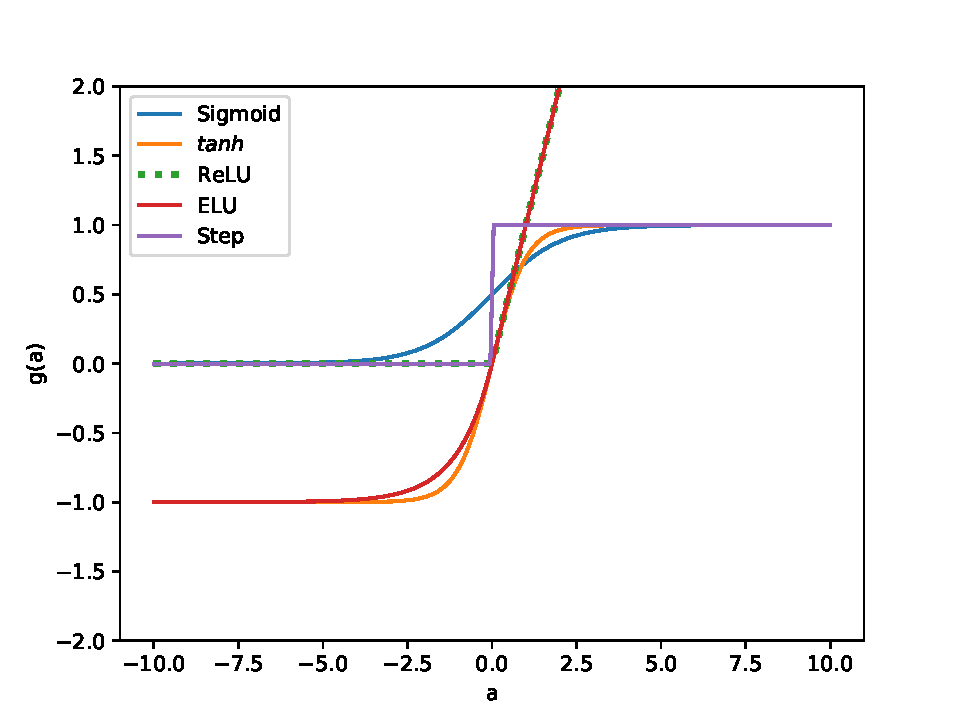
\includegraphics[width=\textwidth,height=\textheight,keepaspectratio]{pics/act_func_fig.pdf}
    \caption{Plot of some of the most used activation functions. \textcolor{red}{Include and refer to code in appendix.}}
    \label{fig:act_funcs}
\end{figure}


\section{Backpropagation} \label{sec:backprop}
As mentioned in section \ref{sec:train_val} we seek to find the hypothesis $\hat{h}^*_S$ that minimizes our empirical loss. For notational convenience we will collect the bias and weights in a parameter vector $\boldsymbol{\theta}$, which can be interpreted as using examples padded with a column of 1's, so that $\boldsymbol{x}\boldsymbol{w}+\boldsymbol{b} = \boldsymbol{x}_{\text{padded}} \boldsymbol{\theta}$. In the case of neural networks $\hat{h}^*_S$ determine the weights used in each neuron as described in section \ref{sec:feedforward_nn}. To obtain these optimal weights we train the neural network by minimizing the gradient of the (perhaps regularized) loss function $J$ with respect to the weights. To learn these weights we use a minimization algorithm like stochastic gradient descent described in section \ref{sec:sgd}. However the gradient of the loss function is not readily available in neural networks as we have to trace back the information back through the network that produced $\hat{y}$ for which we calculate the loss. The solution is an algorithm proposed by \cite{Rumelhart:1986a} called back-propagation or backprop for short.\\
\\
Back-propagation uses the chain rule of calculus, which states that
\begin{equation*}
    \frac{d \, f\lr{g\lr{x}}}{d \, x} = \frac{d \, f\lr{g\lr{x}}}{d \, g \lr{x}} \frac{d \, g\lr{x}}{d \, x}
\end{equation*}
for a real number $x$ and functions $g$ and $f$. This rule can be generalized for a vector $\boldsymbol{x} \in \mathbb{R}^m$
\begin{equation*}
    \frac{\partial f\lr{g\lr{\boldsymbol{x}}}}{\partial x_i} = \sum_j \frac{\partial f\lr{g\lr{\boldsymbol{x}}}}{\partial g(x_j)} \frac{\partial g(x_j)}{\partial x_i}
\end{equation*}
where $g: \mathbb{R}^m \rightarrow \mathbb{R}^n$ and $f: \mathbb{R}^n \rightarrow \mathbb{R}$. In a neural network with 1 hidden layers we find the gradient of the loss function $J(\boldsymbol{\theta})$ (with $\boldsymbol{X}$ and $\boldsymbol{y}$ as implicit inputs to keep notation uncluttered) by
\begin{equation} \label{eq:loss_grad}
    \nabla J\lr{\boldsymbol{\theta}} = \begin{pmatrix}
    \frac{\partial J\lr{f^{\text{out}} \lr{f^{(1)}\lr{\boldsymbol{\theta}}}}}{\partial \theta_1} \\
    \vdots\\
    \frac{\partial J\lr{f^{\text{out}} \lr{f^{(1)}\lr{\boldsymbol{\theta}}}}}{\partial \theta_m}
    \end{pmatrix}
\end{equation}
where each element is found by
\begin{equation} \label{eq:loss_grad_element}
    \frac{\partial J\lr{f^{\text{out}} \lr{f^{(1)}\lr{\boldsymbol{\theta}}}}}{\partial \theta_i} = \frac{\partial J\lr{f^{\text{out}} \lr{f^{(1)}\lr{\boldsymbol{\theta}}}}}{\partial f^{\text{out}} \lr{f^{(1)}\lr{\boldsymbol{\theta}}}} 
    \frac{\partial f^{\text{out}} \lr{f^{(1)}\lr{\boldsymbol{\theta}}}}{\partial f^{(1)}\lr{\boldsymbol{\theta}}} 
    \frac{\partial f^{(1)}\lr{\boldsymbol{\theta}}}{\partial \theta_i}
\end{equation}
which can easily be generalized to networks with more than 1 hidden layer, by using the chain rule in a similar fashion. A computational graph for calculating this in a neural network is shown in figure \ref{fig:backprop_compgraph}. This provides the fundamentals to understand how the gradient is computed in practice. A vector of weights (perhaps chosen by an update of stochastic gradient descent) is sent through the network as shown by algorithm \ref{alg:forward_prop} to provide a loss value. This is called forward-propagation. Then the gradient in equation \ref{eq:loss_grad} is computed using the relation in equation \ref{eq:loss_grad_element} by back-propagation as shown in algorithm \ref{alg:back_prop}. The result of the backpropagation algorithm is gradients on the weights (and biases) that can be directly used for learning the weights that minimizes the gradient on the loss in a stochastic gradient descent algorithm as the one shown in algorithm \ref{alg:sgd}.\\
\\
Some activation functions like the ReLU-function $g(x) = \max \lr{0, x}$ are not differential, which might sound problematic for backpropagation and gradient based learning. However, as mentioned by \cite{Goodfellow-et-al-2016}, gradient descent still performs well enough for these models, partly because training algorithms usually don't arrive at a local minimum of the loss function. This means that we don't expect to get a gradient of $\boldsymbol{0}$, and therefore we can accept that the minimum of the loss function corresponds to points with an undefined gradient. Furthermore \cite{Goodfellow-et-al-2016} mentions that most software return one of the one-sided derivatives, which can be heuristically justified since a computer is subject to numerical error anyway. \\
\\

\begin{figure}
    \centering
    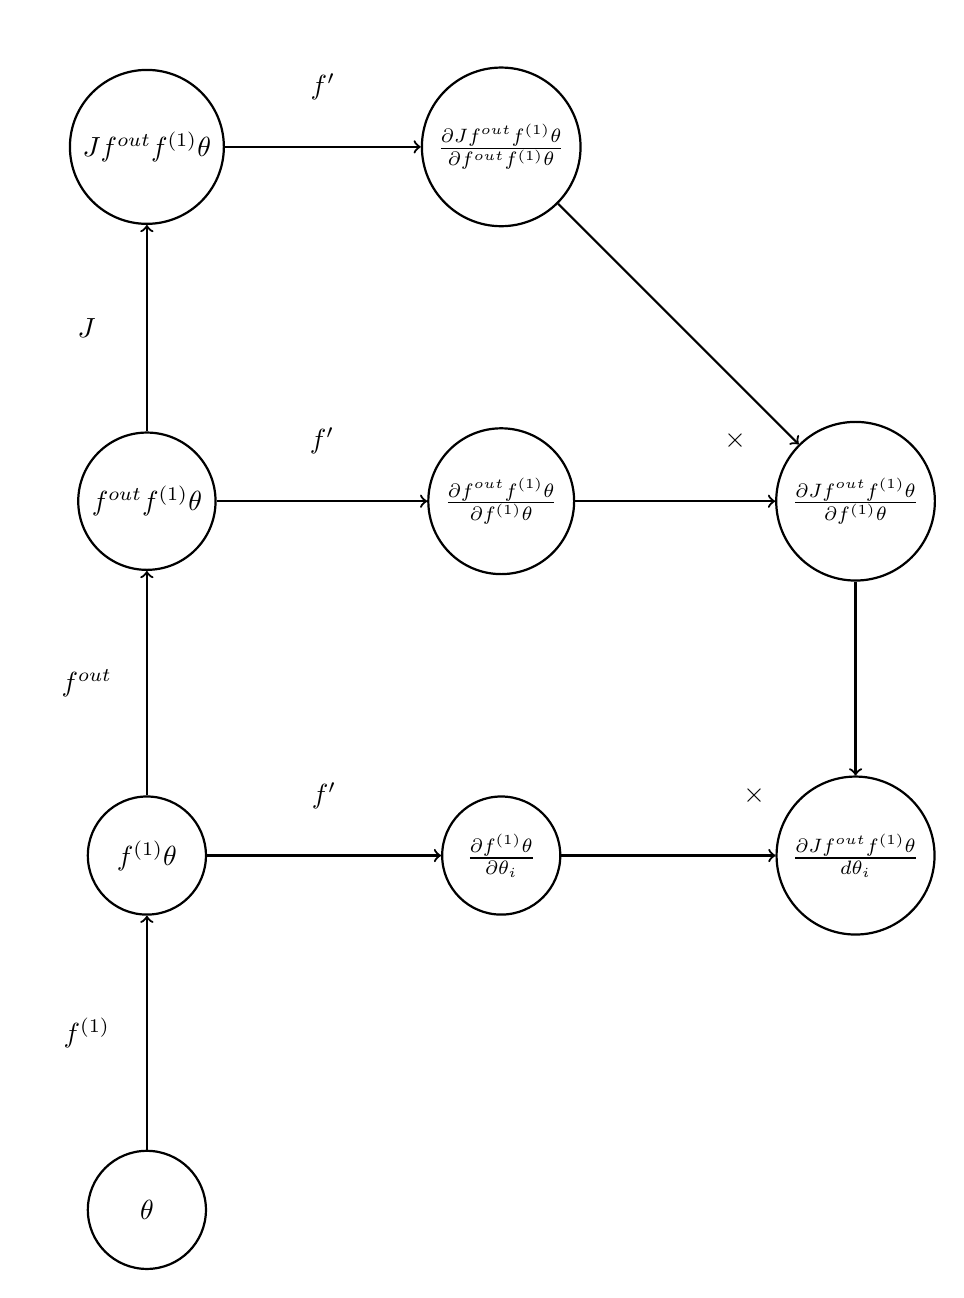
\begin{tikzpicture}[minimum size=1.5cm, node distance={45mm}, thick, main/.style = {draw, circle}] 
        \node[main] (0) {$\boldsymbol{\theta}$}; 
        \node[main] (1) [above of=0]{$f^{(1)} \lr{\boldsymbol{\theta}}$}; 
        \node[main] (2) [right of=1] {$\frac{\partial f^{(1)}\lr{\boldsymbol{\theta}}}{\partial \theta_i}$};
        \node[main] (3) [right of=2] {$\frac{\partial J\lr{f^{\text{out}} \lr{f^{(1)}\lr{\boldsymbol{\theta}}}}}{d \theta_i}$};
        \node[main] (4) [above of=1] {$f^{\text{out}} \lr{ f^{(1)}\lr{\boldsymbol{\theta}}}$};
        \node[main] (5) [right of=4] {$\frac{\partial f^{\text{out}} \lr{f^{(1)}\lr{\boldsymbol{\theta}}}}{\partial f^{(1)}\lr{\boldsymbol{\theta}}} $};
        \node[main] (6) [right of=5] {$\frac{\partial J\lr{f^{\text{out}} \lr{f^{(1)}\lr{\boldsymbol{\theta}}}}}{\partial f^{(1)}\lr{\boldsymbol{\theta}}}$};
        \node[main] (7) [above of=4] {$J \lr{f^{\text{out}} \lr{ f^{(1)}\lr{\boldsymbol{\theta}}}}$};
        \node[main] (8) [right of=7] {$\frac{\partial J\lr{f^{\text{out}} \lr{f^{(1)}\lr{\boldsymbol{\theta}}}}}{\partial f^{\text{out}} \lr{f^{(1)}\lr{\boldsymbol{\theta}}}} $};
        
        \draw[->] (0) -- node[midway, left] {$f^{(1)}$} (1);
        \draw[->] (1) -- node[midway, above] {$f'$} (2);
        \draw[->] (2) -- node[midway, above, pos=0.9] {$\times$} (3);
        \draw[->] (1) -- node[midway, left] {$f^{\text{out}}$} (4);
        \draw[->] (4) -- node[midway, above] {$f'$} (5);
        \draw[->] (5) -- node[midway, above, pos=0.8] {$\times$} (6);
        \draw[->] (6) -- (3);
        \draw[->] (4) -- node[midway, left] {$J$} (7);
        \draw[->] (7) -- node[midway, above] {$f'$} (8);
        \draw[->] (8) -- (6);
    \end{tikzpicture} 
    \caption{Computational graph of calculating the elements of the gradient in equation \ref{eq:loss_grad_element} for the network with 1 hidden layer. $f'$ indicates that the function of the node is derived with regard to its input and $\times$ indicates that the node is a product of the nodes pointing to it. }
    \label{fig:backprop_compgraph}
\end{figure}



\begin{algorithm}\label{alg:forward_prop}
\SetAlgoLined
\KwInput{Number of layers, $l$}
\KwInput{The weight vectors of each layer $\boldsymbol{w}^{(i)}, i \in \lrc{1, \dots, l}$}
\KwInput{The activation functions of each layer, $g^{(i)}, i \in \lrc{1, \dots, l}$}
\KwInput{The example to process, $\boldsymbol{x}$}
\KwInput{The target label for the example, $\boldsymbol{y}$}
\KwOutput{The loss on the example, $J = L\lr{\boldsymbol{\hat{y}}, \boldsymbol{y}} + \lambda \Omega \lr{\boldsymbol{\theta}}$}
 initialize $\boldsymbol{h}^{(0)} = \boldsymbol{x}$ \\
\For{$k = 1, \dots, l$}{
    $\boldsymbol{a}^{(k)} = \boldsymbol{w}^{(k)} \boldsymbol{h}^{(k-1)}$ \\
    $\boldsymbol{h}^{(k)} = g^{(k)} \lr{\boldsymbol{a}^{(k)}}$ \\
}
$\hat{\boldsymbol{y}} = \boldsymbol{h}^{(l)}$ \\
$J = L\lr{\boldsymbol{\hat{y}}, \boldsymbol{y}} + \lambda \Omega \lr{\boldsymbol{\theta}}$ \\
 \caption{Forwardpropagation through a neural network and the computation of the cost function. For simplicity this demonstration uses only a single input example $\boldsymbol{x}$, in practice one typically uses a minibatch of examples. We have also omitted the bias terms for simplicity, as these can be part of the weights $\boldsymbol{w}^{(i)}$ with an example $\boldsymbol{x}$ padded with a column of 1's. The collection of weights are denoted by $\boldsymbol{\theta}$.}
\end{algorithm}

\begin{algorithm}\label{alg:back_prop}
\SetAlgoLined
\KwInput{Same variables as forwardpropagation in algorithm \ref{alg:forward_prop}}
\KwOutput{The gradient of the regularized loss function on the weights, $ \boldsymbol{d} = \nabla_{\boldsymbol{w}}J$}
Perform forward propagation as per algorithm \ref{alg:forward_prop}\\
Computation of the loss-gradient on the output layer:\\
$\boldsymbol{d} \leftarrow \nabla_{\hat{\boldsymbol{y}}} J =  \nabla_{\hat{\boldsymbol{y}}} L\lr{\hat{\boldsymbol{y}}, \boldsymbol{y}}$ \\
\For{$k = l, l-1, \dots, 1$}{
    $\boldsymbol{d} \leftarrow \nabla_{\boldsymbol{a}^{(k)}}J = \boldsymbol{d} \odot g^{(k)'} \lr{\boldsymbol{a}^{(k)}}$\\
    $\nabla_{\boldsymbol{\theta}^{(k)}} J = \boldsymbol{d} \boldsymbol{h}^{(k-1)^\top} + \lambda \nabla_{\boldsymbol{\theta}^{(k)}} \Omega \lr{\boldsymbol{\theta}}$\\
    $\boldsymbol{d} \leftarrow \nabla_{\boldsymbol{h}^{(k-1)}} J = \boldsymbol{\theta}^{(k)^\top} \boldsymbol{d}$\\
}
\caption{Back-propagation}
\end{algorithm}

\section{Early Stopping} \label{sec:early_stopping}
\cite{Goodfellow-et-al-2016} mentions that when we have large models with sufficient capacity to overfit, then we often observe that training error decreases steadily over time, while validation error begins to rise again at some point before ending the training, and that this happens very reliably. This mean that we obtain a better model if we stop training and return the parameters at the point with the lowest validation error. This is the concept of regularizing using early stopping. The algorithm terminates training when no parameters have improved the validation-error over some pre-specified number of iteration called the patience, $p$. The measure of improvement can be controlled by a hyperparameter $\delta$, so that we only constitute an improvement if the decrease in validation error is more than $\delta$. The parameters $\boldsymbol{\theta}$ used for calculating the loss are provided by a training algorithm like ADAM from section \ref{alg:adam} using back-propagation from section \ref{sec:backprop}, while the loss is provided by the network-output for these parameters and the chosen loss function. This procedure is specified more formally in algorithm \ref{alg:es}.\\
\\
One can think of early stopping as a hyperparameter selection algorithm that chooses the number of training steps for the training algorithm. The only significant cost of choosing this parameter automatically with early stopping is running the evaluation of the validation error periodically during training. However this can be done in parallel to the training process, as in Tensorflow where one can run parallel on the GPU. An additional cost is the need to maintain a copy of the optimal parameters, but this is negligible according to \cite{Goodfellow-et-al-2016} since they are written to infrequently and never during the training-algorithm, and since they can preferable be stored in a slower and larger form of memory like in host memory or disk drive. \\
\\
\cite{bishop1995} and \cite{sjoberg_ljung1995} argues that early stopping has the effect of restricting the optimization procedure to a small volume of parameter space in the neighborhood of the initial parameter value. \cite{Goodfellow-et-al-2016} shows with a simple linear model with a quadratic error function and simple linear descent how early stopping is equivalent to $L^2$ regularization in equation \ref{eq:L2_reg}, but that early stopping has the advantage of automatically determining the correct amount of regularization while $L^2$ regularization requires many training experiments with different values of its hyperparameter $\alpha$. 



\begin{algorithm}\label{alg:es}
\SetAlgoLined
\KwInput{The number of steps between evaluations, $n$}
\KwInput{The patience parameter i.e. the number of times of observing worsening validation error before terminating, $p$}
\KwInput{The measure of improvement, $\delta$}
\KwOutput{Parameters when terminating $\boldsymbol{\theta}^{*}$, training step when terminating $i^{*}$}
    initialize $i, j \leftarrow 0$ \\
    initialize $v \leftarrow \infty$\\
    Let $\boldsymbol{\theta}_0$ be the initial parameters\\
    $\boldsymbol{\theta}^* \leftarrow \boldsymbol{\theta}_0$\\
    $i^* \leftarrow i$\\
    \While{$j < p$}{
        Update $\boldsymbol{\theta}$ by running the training algorithm for $n$ steps\\
        $i \leftarrow i + n$\\
        $v' \leftarrow \hat{L}\lr{S_{\text{val}}, \boldsymbol{\theta}}$\\
        \If{$v' < v - \delta$}{
            $j \leftarrow 0$\\
             $\boldsymbol{\theta}^* \leftarrow \boldsymbol{\theta}$\\
            $i^* \leftarrow i$\\
            $v \leftarrow v'$\\
            \Else{
                $j \leftarrow j +1$
            }
        }
    }
 \caption{Early stopping}
\end{algorithm}

